\chapter{Experiments and Results}
The results are reported following the same order as shown in the experiment ledger.
First, the BLIP-2 pair, which tests whether the auxiliary contrastive term adds anything on top of generative fine-tuning.
Then, ScienceQA and A-OKVQA controls, which separate answer-only, rationale-generative, and explanation-aware supervision.
And finally, the last three controls report masking-based visual sensitivity, the Qwen2-VL scale check, and cross-domain transfer.
It is important to note that the results should be viewed in the context of the small-budget protocol, not the leaderboard submissions.

\section{Objective-level comparison}
The objective-level results are shown in Table~\ref{tab:objective_comparison}.
For BLIP-2 on ScienceQA, both objectives yield a slight improvement over the frozen baseline of 0.445.
The contrastive-enhanced run reaches 0.480, while the generative control reaches 0.475.
But the difference is very small and falls within the range of the approximate uncertainty intervals in Table~\ref{tab:uncertainty}.
The same is true for the retrieval diagnostic, where the contrastive-enhanced model has R@1 of 0.010, R@5 of 0.020, R@10 of 0.030, and MRR of 0.0307, which is not a meaningful improvement over the generative control.
Figures~\ref{Fig:BlipObjective} and~\ref{Fig:ContrastiveRetrieval} show these BLIP-2 results.

Qwen2-VL-2B shows stronger results overall.
Rationale-generative fine-tuning scores 0.780 on ScienceQA and 0.790 on A-OKVQA.
Explanation-aware run on A-OKVQA scores 0.795 accuracy, 0.337 ROUGE-L, and 0.087 BLEU.
That is slightly above the generative control, but the difference is small enough that it should be treated as an observed single-run result, not a proven advantage.
The answer-only controls are also strong: 0.800 on ScienceQA and 0.830 on A-OKVQA.
The zero-shot column is reported as a common reference for each model and dataset, not as a separate zero-shot run for every prompt style.
On ScienceQA, the fixed $\alpha=0.50$ explanation-aware run scores 0.765, while the length-aware control scores 0.780, matching the rationale-generative control but still below the answer-only run.
Figure~\ref{Fig:ObjectiveComparison} shows the same controlled comparison visually.

\begin{table*}[!ht]
\centering
\caption{Objective-level results under the controlled protocol. The zero-shot reference is the shared score for the same model and dataset group before the fine-tuning, not a separately recomputed frozen score for every prompt family. Accuracy is multiple-choice accuracy for ScienceQA and A-OKVQA.}
\label{tab:objective_comparison}
\scriptsize
\begin{adjustbox}{max width=\textwidth}
\begin{tabular}{|l|l|l|c|c|c|c|}
\hline
\textbf{Backbone} & \textbf{Dataset} & \textbf{Objective} & \textbf{Zero-shot ref.} & \textbf{Final} & \textbf{ROUGE-L} & \textbf{BLEU} \\ \hline
BLIP-2 OPT-2.7B & ScienceQA & Generative & 0.445 & 0.475 & -- & -- \\
BLIP-2 OPT-2.7B & ScienceQA & Contrastive-enhanced & 0.445 & 0.480 & -- & -- \\
Qwen2-VL-2B & ScienceQA & Answer-only & 0.400 & \textbf{0.800} & -- & -- \\
Qwen2-VL-2B & ScienceQA & Rationale+answer CE & 0.400 & 0.780 & 0.693 & 0.559 \\
Qwen2-VL-2B & ScienceQA & Explanation-aware, $\alpha=0.50$ & 0.400 & 0.765 & 0.643 & 0.493 \\
Qwen2-VL-2B & ScienceQA & Explanation-aware, length-aware & 0.400 & 0.780 & 0.696 & 0.563 \\
Qwen2-VL-2B & A-OKVQA & Answer-only & 0.355 & \textbf{0.830} & -- & -- \\
Qwen2-VL-2B & A-OKVQA & Rationale+answer CE & 0.355 & 0.790 & 0.329 & 0.083 \\
Qwen2-VL-2B & A-OKVQA & Explanation-aware, $\alpha=0.50$ & 0.355 & 0.795 & 0.337 & 0.087 \\
Qwen2-VL-2B & A-OKVQA & Explanation-aware, length-aware & 0.355 & 0.790 & 0.330 & 0.083 \\ \hline
\end{tabular}
\end{adjustbox}
\end{table*}

\begin{table*}[!ht]
\centering
\caption{Approximate uncertainty for selected accuracy-style headline metrics. These intervals use the generated normal-approximation standard errors for capped evaluation sets, so they are a caution about small observed differences rather than a replacement for multi-seed testing.}
\label{tab:uncertainty}
\scriptsize
\begin{adjustbox}{max width=\textwidth}
\begin{tabular}{|l|l|c|c|c|}
\hline
\textbf{Run} & \textbf{Metric} & \textbf{Eval cap} & \textbf{Score} & \textbf{Approx. 95\% CI} \\ \hline
BLIP-2 generative ScienceQA & MC accuracy & 200 & 0.475 & 0.406--0.544 \\
BLIP-2 contrastive ScienceQA & MC accuracy & 200 & 0.480 & 0.411--0.549 \\
ScienceQA answer-only & MC accuracy & 200 & 0.800 & 0.745--0.855 \\
ScienceQA rationale+answer CE & MC accuracy & 200 & 0.780 & 0.723--0.837 \\
ScienceQA explanation-aware, $\alpha=0.50$ & MC accuracy & 200 & 0.765 & 0.706--0.824 \\
ScienceQA explanation-aware, length-aware & MC accuracy & 200 & 0.780 & 0.723--0.837 \\
A-OKVQA answer-only & MC accuracy & 200 & 0.830 & 0.778--0.882 \\
A-OKVQA rationale+answer CE & MC accuracy & 200 & 0.790 & 0.734--0.847 \\
A-OKVQA explanation-aware, $\alpha=0.50$ & MC accuracy & 200 & 0.795 & 0.739--0.851 \\
Qwen2-VL-7B ScienceQA, $\alpha=0.50$ & MC accuracy & 200 & 0.885 & 0.841--0.929 \\ \hline
\end{tabular}
\end{adjustbox}
\end{table*}

\begin{figure}[!ht]
\centerline{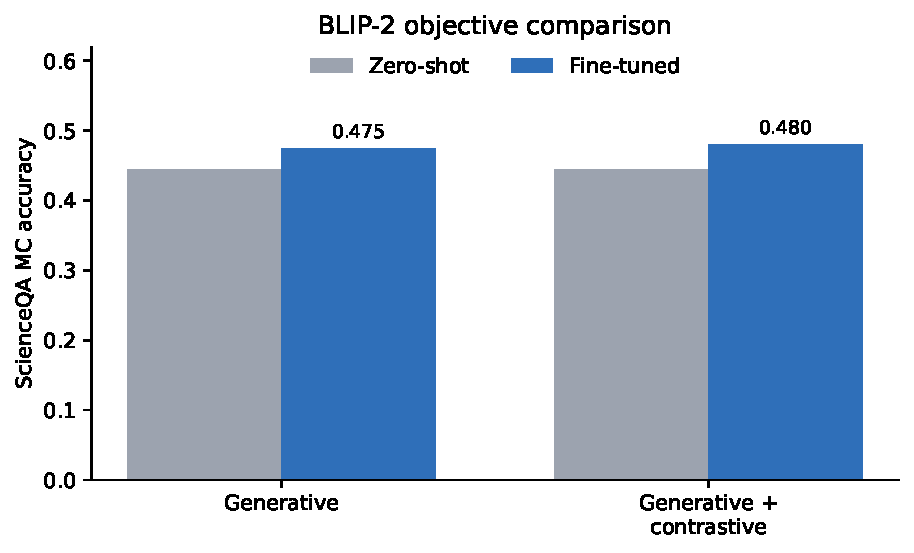
\includegraphics[width=0.82\linewidth]{./Figures/generated/blip2_objective}}
\caption{BLIP-2 generative and contrastive-enhanced ScienceQA results.
Both runs improve over the frozen baseline, with only a small observed gain from the auxiliary contrastive term.}
\label{Fig:BlipObjective}
\end{figure}

\begin{figure}[!ht]
\centerline{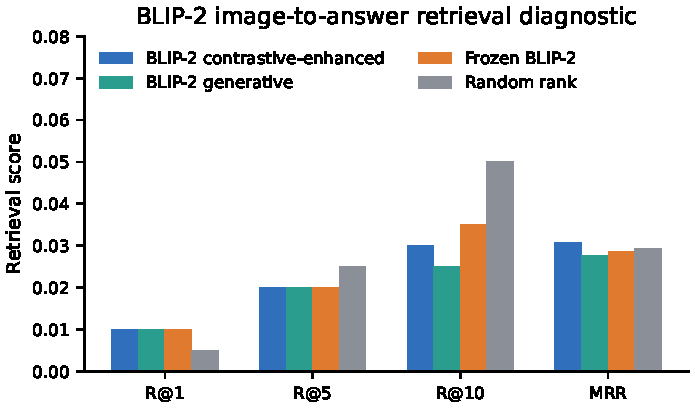
\includegraphics[width=0.82\linewidth]{./Figures/generated/contrastive_retrieval}}
\caption{BLIP-2 image-to-answer retrieval diagnostic.
The analysis reports frozen BLIP-2, BLIP-2 generative, BLIP-2 contrastive-enhanced, and random-rank controls so the contrastive branch is not interpreted without a reference point.}
\label{Fig:ContrastiveRetrieval}
\end{figure}

\begin{figure}[!ht]
\centerline{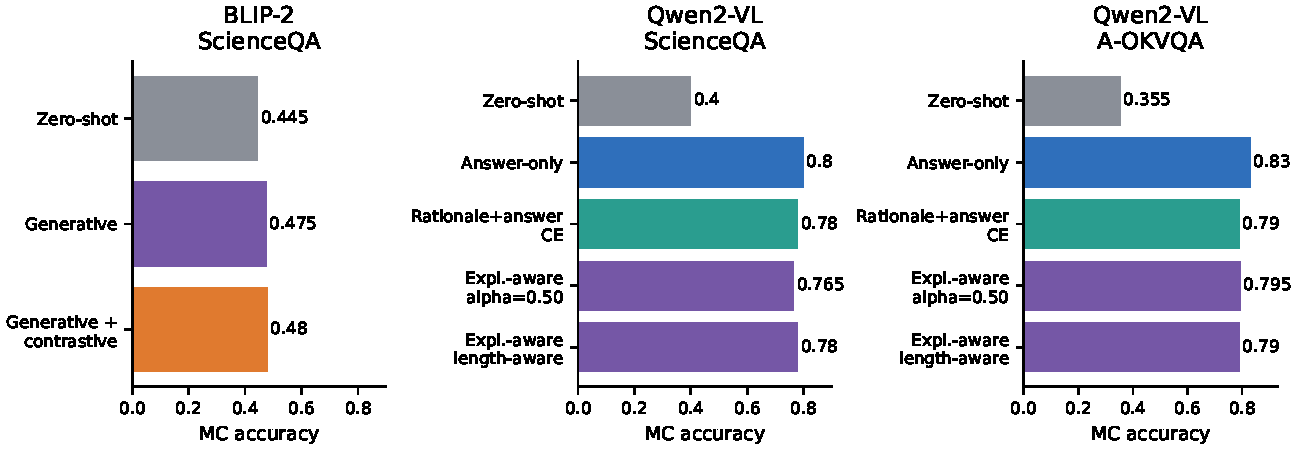
\includegraphics[width=\linewidth]{./Figures/generated/controlled_strategy_comparison}}
\caption{Controlled strategy comparison for BLIP-2 and Qwen2-VL.
The figure shows zero-shot, answer-only, rationale-generative, explanation-aware, and contrastive variants where those controls are available.}
\label{Fig:ObjectiveComparison}
\end{figure}

\FloatBarrier

\section{Effect of explanation-aware training}
Table~\ref{tab:alpha_sweep} and Figure~\ref{Fig:AlphaSweep} show the ScienceQA fixed-$\alpha$ sweep.
Here $\alpha$ is the answer-span weight from Equation~\ref{Eq:Loss}.
Fine-tuning raises accuracy from the 0.400 zero-shot reference into the 0.690--0.780 range.
The best fixed setting is low answer weight: $\alpha=0.10$, which reaches 0.780.
As $\alpha$ moves toward the answer-heavy end, accuracy drops to 0.690 at $\alpha=0.75$ and 0.695 at $\alpha=1.00$.
The same pattern is observed on the rationale metrics.
ROUGE-L and BLEU also reach the maximum at $\alpha=0.10$ (0.695 and 0.566), then decline as $\alpha$ increases.
At $\alpha=1.00$, only the answer span is supervised inside a target but the rationale part is still included in the target template, although it is not weighted in the loss. Hence, the rationale metrics are not computed in that case.

The $\alpha=0.10$ run matches the rationale-generative and length-aware controls on accuracy.
The $\alpha=1.00$ run should not be confused with a true answer-only run, because the target template in that case still contains the rationale part,
even though that rationale span is not included in the loss.
The answer-only control on ScienceQA is trained with a target that contains only the answer part of the template, reaches 0.800,
which is above the best fixed-$\alpha$ run and the rationale-generative control.
All of these comparisons use one seed, 2{,}000 training examples, and 200 evaluation examples, so they show observed behaviour rather than final statistical proof.

\begin{table}[!ht]
\centering
\caption{Explanation-aware fixed-$\alpha$ sweep on ScienceQA (Qwen2-VL-2B, QLoRA, 2{,}000 train / 200 eval, single seed). The coefficient $\alpha$ weights the answer span in Equation~\ref{Eq:Loss}: $\alpha=1$ is answer-span-only within the rationale target and $\alpha=0$ is explanation-span-only. The zero-shot and rationale-generative rows are references. Random-choice accuracy is 0.354. The best fixed $\alpha$ is shown in bold.}
\label{tab:alpha_sweep}
\begin{tabular}{|l|c|c|c|}
\hline
\textbf{Variant ($\alpha$)} & \textbf{MC accuracy} & \textbf{ROUGE-L} & \textbf{BLEU} \\ \hline
Zero-shot (frozen) & 0.400 & -- & -- \\
Rationale+answer CE & \textbf{0.780} & 0.693 & 0.559 \\ \hline
$\alpha=0.00$ (explanation-only) & 0.725 & 0.417 & 0.299 \\
$\alpha=0.10$ & \textbf{0.780} & \textbf{0.695} & \textbf{0.566} \\
$\alpha=0.25$ & 0.775 & 0.686 & 0.548 \\
$\alpha=0.50$ & 0.765 & 0.643 & 0.493 \\
$\alpha=0.75$ & 0.690 & 0.604 & 0.443 \\
$\alpha=1.00$ (answer-span only) & 0.695 & -- & -- \\ \hline
\end{tabular}
\end{table}

\begin{figure}[!ht]
\centerline{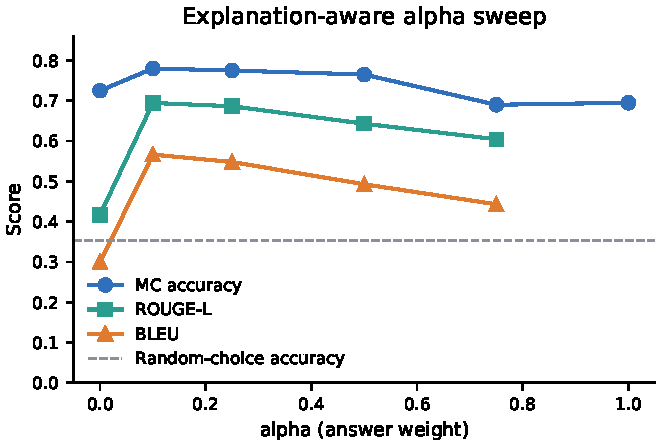
\includegraphics[width=0.82\linewidth]{./Figures/generated/alpha_sweep}}
\caption{Fixed-alpha explanation-aware sweep on ScienceQA.
Answer accuracy peaks at the low-answer-weight setting and declines toward both extremes inside the rationale-plus-answer target.
Explanation quality (ROUGE-L, BLEU) peaks at the same point and falls as $\alpha$ increases.
Series are distinguished by marker shape and line style; the dashed grey line marks random-choice accuracy. Single seed.}
\label{Fig:AlphaSweep}
\end{figure}

\FloatBarrier

\section{Domain-level behaviour}
Table~\ref{tab:domain_results} and Figure~\ref{Fig:CrossDomain} represent the results for the selected in-domain runs.
Fixed $\alpha=0.50$ is used for the ScienceQA row, so that it matches the selected domain comparison.
The stronger $\alpha=0.10$ and length-aware settings are reported separately in the sweep above.
A-OKVQA rises from 0.355 to 0.795 accuracy against the zero-shot reference.
The VQAv2 subset rises from 0.350 to 0.730 VQA accuracy.
ChartQA reaches 0.655 relaxed accuracy, with exact match at 0.410.
DocVQA reaches 0.905 ANLS and 0.855 exact match.
Although the DocVQA score is strong in this run, it should be read carefully, because the examples are mostly short extractive answers, the training setup is answer-only fallback rather than gold-rationale supervision, and the split audit cannot prove document-level disjointness beyond the native IDs exposed by the loader.

\begin{table*}[!ht]
\centering
\caption{Domain-level results for the completed Qwen2-VL-2B runs. Each domain uses its native headline metric: multiple-choice accuracy for ScienceQA and A-OKVQA, relaxed accuracy for ChartQA, ANLS for DocVQA, and VQA accuracy for the VQAv2 subset.}
\label{tab:domain_results}
\scriptsize
\begin{adjustbox}{max width=\textwidth}
\begin{tabular}{|l|l|l|c|c|c|}
\hline
\textbf{Domain} & \textbf{Dataset} & \textbf{Objective} & \textbf{Zero-shot ref.} & \textbf{Final} & \textbf{Secondary metric} \\ \hline
Science & ScienceQA & Explanation-aware, $\alpha=0.50$ & 0.400 & 0.765 & ROUGE-L 0.643, BLEU 0.493 \\
Commonsense & A-OKVQA & Explanation-aware, $\alpha=0.50$ & 0.355 & 0.795 & ROUGE-L 0.337, BLEU 0.087 \\
Charts & ChartQA & Answer-only fallback & 0.335 & 0.655 & Exact match 0.410 \\
Documents & DocVQA & Answer-only fallback & 0.349 & 0.905 & Exact match 0.855 \\
Natural images & VQAv2 subset & Answer-only fallback & 0.350 & 0.730 & Exact match 0.350 $\rightarrow$ 0.730 \\ \hline
\end{tabular}
\end{adjustbox}
\end{table*}

\begin{figure}[!ht]
\centerline{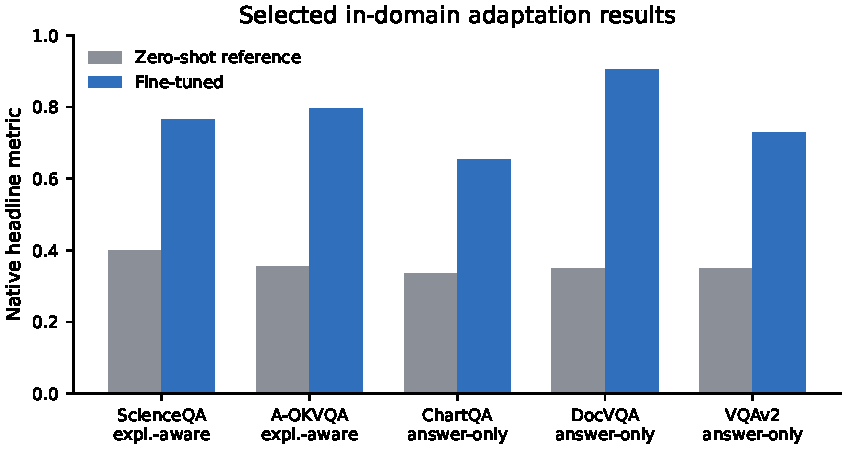
\includegraphics[width=0.82\linewidth]{./Figures/generated/cross_domain}}
\caption{In-domain adaptation results for the selected completed Qwen2-VL-2B domain runs.
The comparison mixes rationale-supervised ScienceQA/A-OKVQA rows with answer-only fallback rows for domains without gold rationales, so it should not be read as an explanation-aware effect across all domains.}
\label{Fig:CrossDomain}
\end{figure}

\FloatBarrier

\section{Faithfulness and hallucination analysis}
Evidence-masking drift is shown in Table~\ref{tab:faithfulness} and Figure~\ref{Fig:Faithfulness}.
Each value is averaged over 30 evaluation examples.
Higher positive drift means that the model produced lower probability for the real answer when the masked region was occluded, meaning that the model relied on that region as evidence for the answer.
The strongest evidence sensitivity is observed in the structured tasks: DocVQA at 0.375, ChartQA at 0.224, and VQAv2 at 0.111.
ScienceQA and A-OKVQA are much lower, with the ScienceQA answer-only adapter as the main exception at 0.0898.

Low ScienceQA drift is understandable, because many ScienceQA items could be partly answered based on the question and the answer choices using the learned facts, the relevant visual evidence can be spread across the image, and a coarse mask may miss the regions the model actually uses.
Explanation supervision does not create a clean drift pattern in this run.
The $\alpha=0.10$ setting gives 0.0223, $\alpha=0.50$ gives 0.0197, and answer-span-only $\alpha=1.00$ gives 0.0149, even though that run has no supervised rationale metric.
On A-OKVQA, the explanation-aware run has slightly higher drift than the generative control (0.0271 versus 0.0245), but both intervals are wide.
Hence, the evidence-masking results do not demonstrate that the explanation-aware training yields a stronger visual sensitivity than the rationale-generative control.
Figure~\ref{Fig:MaskingExample} shows one saved masking example.

\begin{table}[!ht]
\centering
\caption{Evidence-masking drift by completed run. Higher values indicate stronger sensitivity to masked visual evidence. The intervals are approximate 95\% intervals from the generated masking artifact.}
\label{tab:faithfulness}
\scriptsize
\begin{adjustbox}{max width=\textwidth}
\begin{tabular}{|l|c|c|c|}
\hline
\textbf{Run} & \textbf{Mean drift} & \textbf{Approx. 95\% CI} & \textbf{Examples} \\ \hline
ScienceQA answer-only & 0.0898 & 0.0197--0.1830 & 30 \\
ScienceQA rationale+answer CE & 0.0217 & -0.0100--0.0582 & 30 \\
ScienceQA $\alpha=0.10$ & 0.0223 & -0.0080--0.0568 & 30 \\
ScienceQA $\alpha=0.50$ & 0.0197 & -0.0119--0.0552 & 30 \\
ScienceQA answer-span-only $\alpha=1.00$ & 0.0149 & -0.0274--0.0638 & 30 \\
A-OKVQA rationale+answer CE & 0.0245 & -0.0236--0.0726 & 30 \\
A-OKVQA explanation-aware & 0.0271 & -0.0075--0.0627 & 30 \\
ChartQA answer-only fallback & 0.2237 & 0.1419--0.3140 & 30 \\
DocVQA answer-only fallback & 0.3749 & 0.2770--0.4960 & 30 \\
VQAv2 answer-only fallback & 0.1109 & 0.0274--0.2408 & 30 \\
Qwen2-VL-7B ScienceQA $\alpha=0.50$ & 0.0114 & -0.0059--0.0260 & 30 \\ \hline
\end{tabular}
\end{adjustbox}
\end{table}

\begin{figure}[!ht]
\centerline{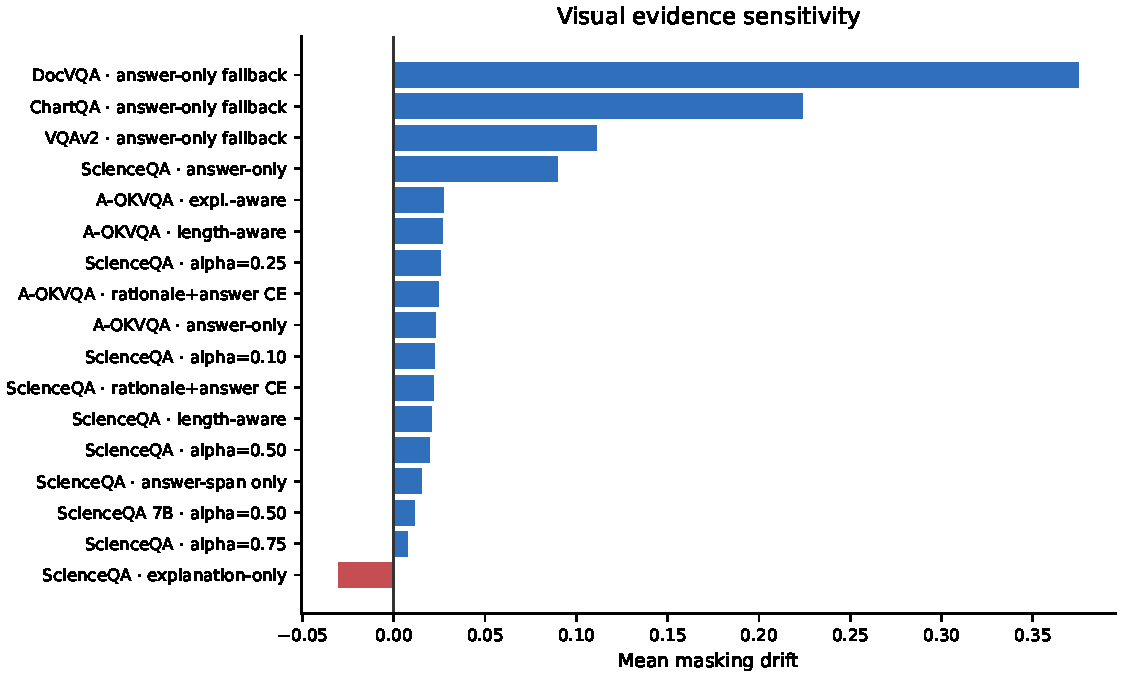
\includegraphics[width=0.82\linewidth]{./Figures/generated/faithfulness}}
\caption{Mean evidence-masking drift across completed runs.
Structured document and chart runs show much stronger visual sensitivity than the rationale-rich ScienceQA and A-OKVQA runs, but stronger drift does not automatically imply better answer accuracy.}
\label{Fig:Faithfulness}
\end{figure}

\IfFileExists{./Figures/generated/masking_example_chartqa_clean.pdf}{
\begin{figure*}[!ht]
\centerline{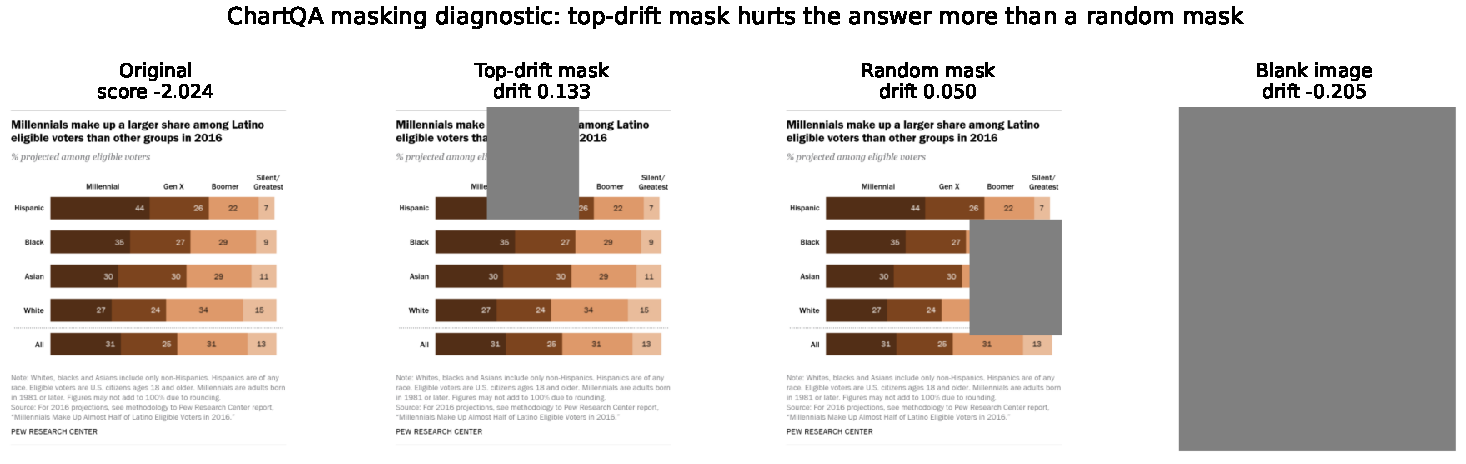
\includegraphics[width=\linewidth]{./Figures/generated/masking_example_chartqa_clean}}
\caption{Example masking diagnostic for a ChartQA answer-only fallback run.
The pipeline saves the original image, the top-drift mask, a random-region mask, and a blank-image control, together with the full-image and masked answer scores.
This figure is used as an evidence-sensitivity example, not as proof that a generated rationale is faithful.}
\label{Fig:MaskingExample}
\end{figure*}
}{}

\FloatBarrier

\section{Efficiency and scale trade-offs}
The comparison between Qwen2-VL-2B and Qwen2-VL-7B using the same ScienceQA explanation-aware setting ($\alpha=0.50$) is shown in Table~\ref{tab:scale} and Figure~\ref{Fig:Scale}.
The larger model shows a clear improvement in the completed experiments.
Accuracy rises from 0.765 to 0.885.
ROUGE-L moves from 0.643 to 0.738, and BLEU moves from 0.493 to 0.637.
The comparison is still within the same parameter-efficient setting, because both runs are fine-tuned using the same QLoRA setup.
However, the logs do not include the exact GPU hours or memory usage for each run, so we treat this as a scale comparison rather than a full efficiency benchmark.

\begin{table}[!ht]
\centering
\caption{Qwen2-VL scale comparison on ScienceQA with the same explanation-aware objective ($\alpha=0.50$).}
\label{tab:scale}
\begin{tabular}{|l|c|c|c|}
\hline
\textbf{Model} & \textbf{MC accuracy} & \textbf{ROUGE-L} & \textbf{BLEU} \\ \hline
Qwen2-VL-2B & 0.765 & 0.643 & 0.493 \\
Qwen2-VL-7B & \textbf{0.885} & \textbf{0.738} & \textbf{0.637} \\ \hline
\end{tabular}
\end{table}

\begin{figure}[!ht]
\centerline{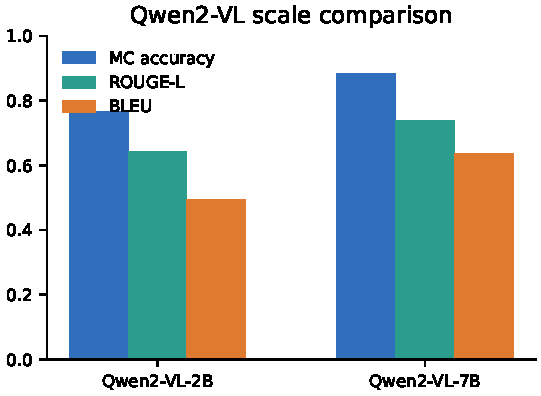
\includegraphics[width=0.82\linewidth]{./Figures/generated/scale_comparison}}
\caption{Scale comparison for the fixed ScienceQA explanation-aware setting.
Moving from Qwen2-VL-2B to Qwen2-VL-7B improves both answer accuracy and rationale-overlap metrics.}
\label{Fig:Scale}
\end{figure}

\FloatBarrier

\section{Cross-domain transfer}
Table~\ref{tab:transfer} and Figure~\ref{Fig:Transfer} present the transfer matrix from training domain to evaluation domain.
Each column uses the metric of the target dataset, so values should be compared within a column rather than across a row.
The matrix keeps answer-only, rationale-generative, and explanation-aware sources separate.
This table is a transfer probe, not a replacement for the in-domain results.
Since the transfer evaluator might use a different prompt family than the in-domain evaluation (e.g., answer-only transfer evaluated with an answer-only prompt), the diagonal values may not be exactly the same as the in-domain table.

The transfer results are not explained by the dataset domain alone, meaning that the training objective also influences how well a model transfers.
The ScienceQA answer-only adapter transfers well, reaching 0.805 on A-OKVQA, 0.645 on ChartQA, 0.703 on DocVQA, and 0.630 on VQAv2.
The ScienceQA rationale-generative and explanation-aware adapters are above random baselines, but they transfer less well to ChartQA, DocVQA, and VQAv2 compared to the answer-only adapter.
For A-OKVQA sources, rationale-generative training gives the strongest DocVQA transfer in that group (0.764), while answer-only training gives the strongest VQAv2 transfer (0.700).
DocVQA is strongest in-domain at 0.910, and the document-trained adapter also transfers well to ChartQA at 0.685.
Overall, transfer depends on both the target domain and the source objective.

\begin{table*}[!ht]
\centering
\caption{Cross-domain transfer matrix. Rows indicate the training domain and columns indicate the evaluation domain. Each column uses the target domain's headline metric, so values are best compared within a column.}
\label{tab:transfer}
\scriptsize
\begin{adjustbox}{max width=\textwidth}
\begin{tabular}{|l|ccccc|}
\hline
\textbf{Trained on} & \textbf{ScienceQA} & \textbf{A-OKVQA} & \textbf{ChartQA} & \textbf{DocVQA} & \textbf{VQAv2} \\ \hline
ScienceQA answer-only & 0.800 & 0.805 & 0.645 & 0.703 & 0.630 \\
ScienceQA rationale CE & 0.780 & 0.760 & 0.450 & 0.559 & 0.300 \\
ScienceQA explanation-aware & 0.740 & 0.765 & 0.460 & 0.491 & 0.410 \\
A-OKVQA answer-only & 0.690 & 0.825 & 0.635 & 0.677 & 0.700 \\
A-OKVQA rationale CE & 0.665 & 0.790 & 0.645 & 0.764 & 0.600 \\
A-OKVQA explanation-aware & 0.680 & 0.795 & 0.615 & 0.763 & 0.640 \\
ChartQA answer-only & 0.420 & 0.415 & 0.660 & 0.831 & 0.680 \\
DocVQA answer-only & 0.450 & 0.435 & 0.685 & 0.910 & 0.660 \\
VQAv2 answer-only & 0.440 & 0.575 & 0.660 & 0.716 & 0.730 \\ \hline
\end{tabular}
\end{adjustbox}
\end{table*}

\begin{figure}[!ht]
\centerline{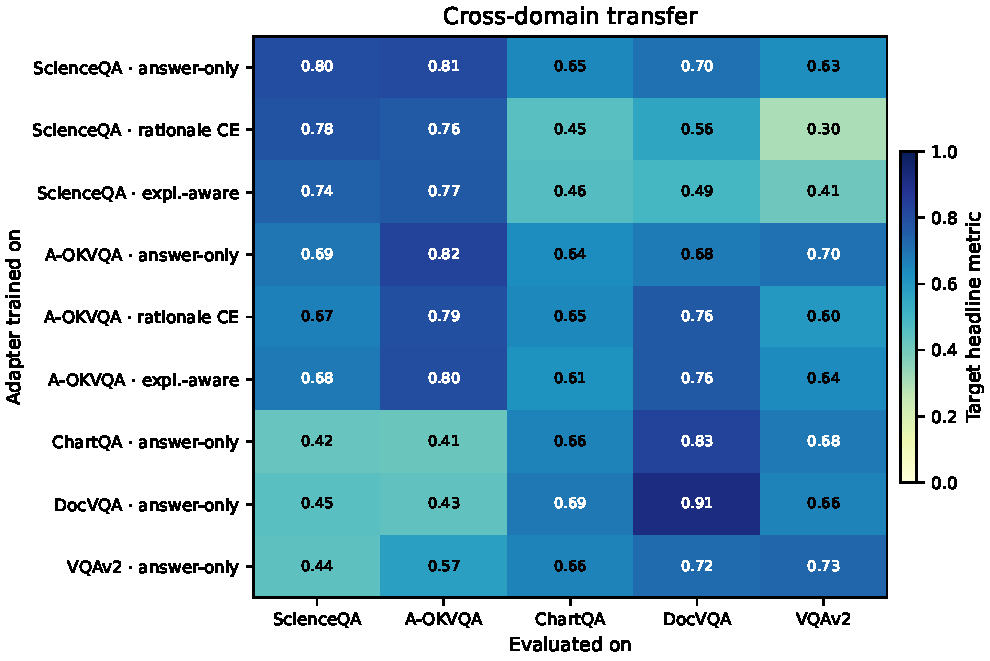
\includegraphics[width=0.76\linewidth]{./Figures/generated/transfer_matrix}}
\caption{Cross-domain transfer heatmap.
The strongest non-diagonal transfer is not always from the visually closest domain.
Answer-only ScienceQA transfers strongly to A-OKVQA, while answer-only document and chart adapters transfer strongly to several open-ended targets.}
\label{Fig:Transfer}
\end{figure}

\FloatBarrier
